%---------- Inleiding ---------------------------------------------------------

\section{Inleiding}%
\label{sec:inleiding}

Match- en spelerstatistieken zijn van essentieel belang in de sportwereld, maar bij Lindemans Aalst is dit nog zeer tijdrovend. Tijdens wedstrijden worden statistieken handmatig bijgehouden, terwijl er tijdens trainingen zelfs geen gegevens worden verzameld. Dit handmatige proces is niet alleen inefficiënt, maar kan ook leiden tot inconsistenties in de data. Automatisering van statistiekenregistratie biedt potentieel voor een systeem dat in staat is real-time statistieken vast te leggen, zowel tijdens wedstrijden als trainingen, wat resulteert in een meer efficiënte en betrouwbare dataverzameling. Daarom dus: "Welke bestaande AI-oplossing voor het automatiseren van volleybalstatistieken biedt de meeste voordelen voor Lindemans Aalst, zowel tijdens wedstrijden als trainingen?". Het zou daarom beter zijn dat de statistieken worden geautomatiseerd. Dit zou ervoor zorgen dat er minder fouten aanwezig zijn en dat de statistieken sneller beschikbaar zijn. Dit zou er dan weer voor zorgen dat de coaches sneller en beter beslissingen kunnen maken.

%---------- Stand van zaken ---------------------------------------------------

\section{Literatuurstudie}%
\label{sec:literatuurstudie}

Hier beschrijf je de \emph{state-of-the-art} rondom je gekozen onderzoeksdomein, d.w.z.\ een inleidende, doorlopende tekst over het onderzoeksdomein van je bachelorproef. Je steunt daarbij heel sterk op de professionele \emph{vakliteratuur}, en niet zozeer op populariserende teksten voor een breed publiek. Wat is de huidige stand van zaken in dit domein, en wat zijn nog eventuele open vragen (die misschien de aanleiding waren tot je onderzoeksvraag!)?

Je mag de titel van deze sectie ook aanpassen (literatuurstudie, stand van zaken, enz.). Zijn er al gelijkaardige onderzoeken gevoerd? Wat concluderen ze? Wat is het verschil met jouw onderzoek?

Verwijs bij elke introductie van een term of bewering over het domein naar de vakliteratuur, bijvoorbeeld~\autocite{Hykes2013}! Denk zeker goed na welke werken je refereert en waarom.

Draag zorg voor correcte literatuurverwijzingen! Een bronvermelding hoort thuis \emph{binnen} de zin waar je je op die bron baseert, dus niet er buiten! Maak meteen een verwijzing als je gebruik maakt van een bron. Doe dit dus \emph{niet} aan het einde van een lange paragraaf. Baseer nooit teveel aansluitende tekst op eenzelfde bron.

Als je informatie over bronnen verzamelt in JabRef, zorg er dan voor dat alle nodige info aanwezig is om de bron terug te vinden (zoals uitvoerig besproken in de lessen Research Methods).

% Voor literatuurverwijzingen zijn er twee belangrijke commando's:
% \autocite{KEY} => (Auteur, jaartal) Gebruik dit als de naam van de auteur
%   geen onderdeel is van de zin.
% \textcite{KEY} => Auteur (jaartal)  Gebruik dit als de auteursnaam wel een
%   functie heeft in de zin (bv. ``Uit onderzoek door Doll & Hill (1954) bleek
%   ...'')

Je mag deze sectie nog verder onderverdelen in subsecties als dit de structuur van de tekst kan verduidelijken.

%---------- Methodologie ------------------------------------------------------
\section{Methodologie}%
\label{sec:methodologie}

Elke week die beschreven wordt bestaat uit 1 volledige dag werk aan de bachelorproef.
\subsection{Fase 1: Literatuurstudie}
De literatuurstudie is bedoeld om inzicht te krijgen in de huidige stand van zaken met betrekking tot AI-systemen die geschikt zijn voor het verzamelen en analyseren van sportstatistieken. Deze fase omvat een grondige analyse van academische publicaties, whitepapers en technische documentatie van bekende AI-tools, zoals Hudl, DataVolley, Second Spectrum en Balltime AI. De focus ligt hierbij op het evalueren van nauwkeurigheid, snelheid, schaalbaarheid en kosten van deze systemen, aangezien deze factoren belangrijk zijn voor de toepassing binnen Lindemans Aalst. Aan het einde van deze fase wordt een overzichtsrapport opgesteld met de bevindingen, waarin ook een vergelijkingstabel wordt opgenomen die de sterke en zwakke punten van elk systeem schetst. Dit rapport vormt de basis voor de selectie van systemen die in latere fases verder onderzocht zullen worden. Deze fase duurt 2 weken.
\subsection{Fase 2: Interviews en requirementsanalyse}
In de tweede fase, die 1 week duurt, worden gestructureerde interviews afgenomen met de coaches, data-analisten en technische staf van Lindemans Aalst. Het doel van deze interviews is om een duidelijk beeld te krijgen van de functionele en technische eisen die de club stelt aan een geautomatiseerd statistiekensysteem. De requirements-analyse richt zich op de statistieken die essentieel zijn voor de club en op specifieke analyses die coaches tijdens wedstrijden en trainingen nodig hebben. De inzichten uit deze gesprekken worden verwerkt in een requirementsdocument, dat de functionele en technische vereisten vastlegt. Dit document vormt een referentiepunt voor de vergelijkende analyse van de AI-systemen in de volgende fase.
\subsection{Fase 3: Vergelijkende studie van AI-systemen}
In deze 3 weken durende fase worden de geselecteerde AI-systemen geëvalueerd op basis van nauwkeurigheid, snelheid en gebruiksgemak, om objectief te bepalen welke oplossing het best aansluit bij de eisen van Lindemans Aalst. Hiervoor wordt gebruikgemaakt van eerder verzamelde datasets van match- en trainingsgegevens. De systemen worden getest op hun vermogen om deze data nauwkeurig en snel te verwerken en de resultaten worden vergeleken met de handmatig geregistreerde data. Deze evaluatie wordt gepresenteerd in een rapport met grafieken en tabellen die de prestaties van elk systeem visueel weergeven. Het rapport bevat ook een concrete aanbeveling van het systeem dat het meest geschikt lijkt voor implementatie, op basis van de vergelijking.
\subsection{Fase 4: Proof of concept en praktijktest}
Na de vergelijkende studie wordt het aanbevolen systeem geïmplementeerd als proof of concept (PoC) bij Lindemans Aalst. Deze praktijktest van 3 weken heeft als doel te valideren of het systeem daadwerkelijk voldoet aan de functionele en technische eisen van de club. Gedurende deze periode verzamelt het systeem automatisch gegevens tijdens trainingen en wedstrijden, zodat coaches en analisten het gebruiksgemak en de nauwkeurigheid van de automatisering kunnen evalueren. De prestaties van het PoC-systeem worden vergeleken met handmatig geregistreerde gegevens en de feedback van de coaches over de gebruiksvriendelijkheid wordt verzameld. Aan het einde van deze fase wordt een validatierapport opgesteld, waarin de kwantitatieve resultaten van het geautomatiseerde systeem zijn opgenomen, evenals eventuele aanbevelingen voor optimalisatie.
\subsection{Fase 5: Analyse en eindrapport}
In de laatste fase, die nog 2 weken zal duren, worden de resultaten van het onderzoek geanalyseerd en samengebracht in een eindrapport. Dit rapport bevat een grondige analyse van de prestaties van het PoC-systeem en conclusies over de mate waarin het systeem de doelstellingen van Lindemans Aalst ondersteunt. De data uit de eerdere fases worden statistisch geanalyseerd om objectieve conclusies te trekken over de impact van automatisering op de nauwkeurigheid en snelheid van statistiekenregistratie. Het rapport bevat tevens aanbevelingen voor de club over de definitieve implementatie van het AI-systeem en suggesties voor toekomstige optimalisaties.

\begin{figure}[ht]
  \centering
  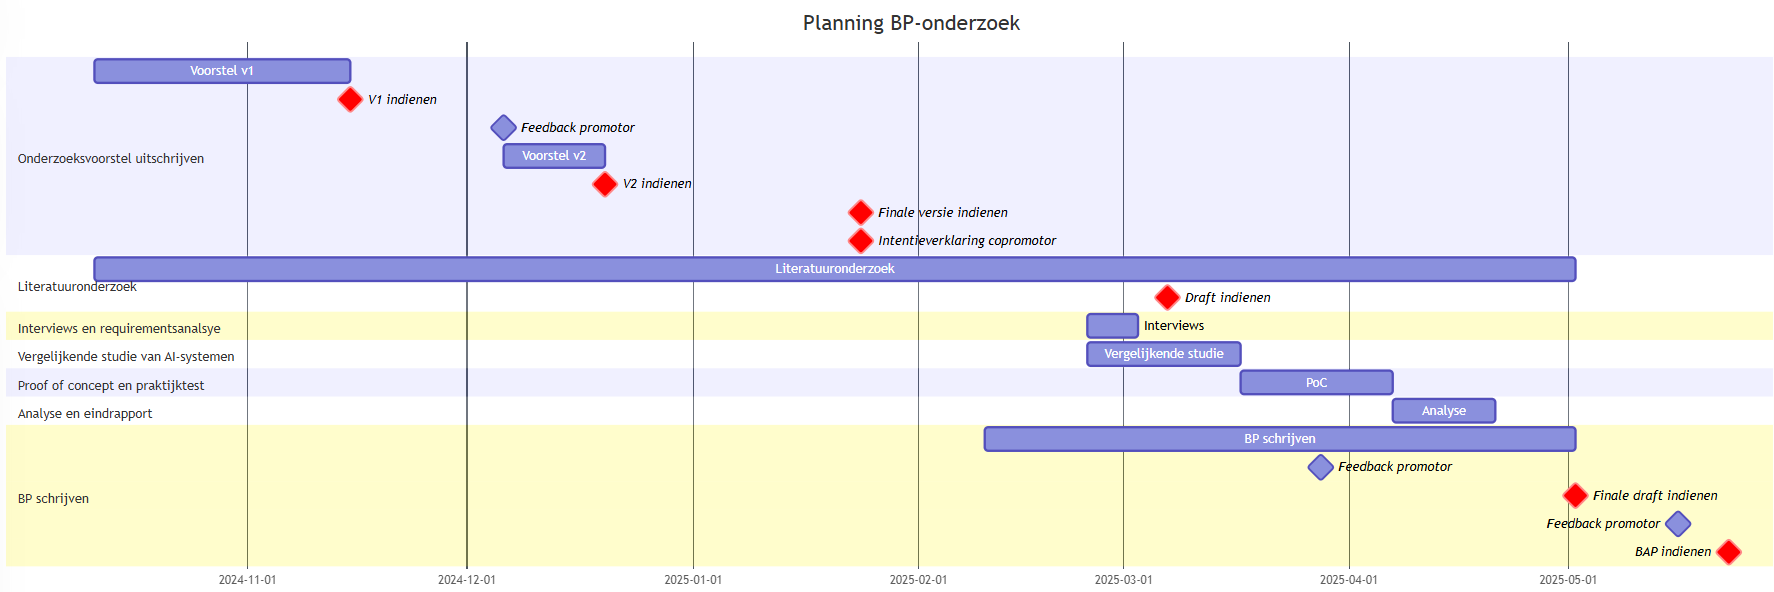
\includegraphics[width=0.5\textwidth]{img/gantt.png}
  \caption{\label{fig:gantt}Gantt planning bachelorproef}
\end{figure}

\begin{figure}[ht]
  \centering
  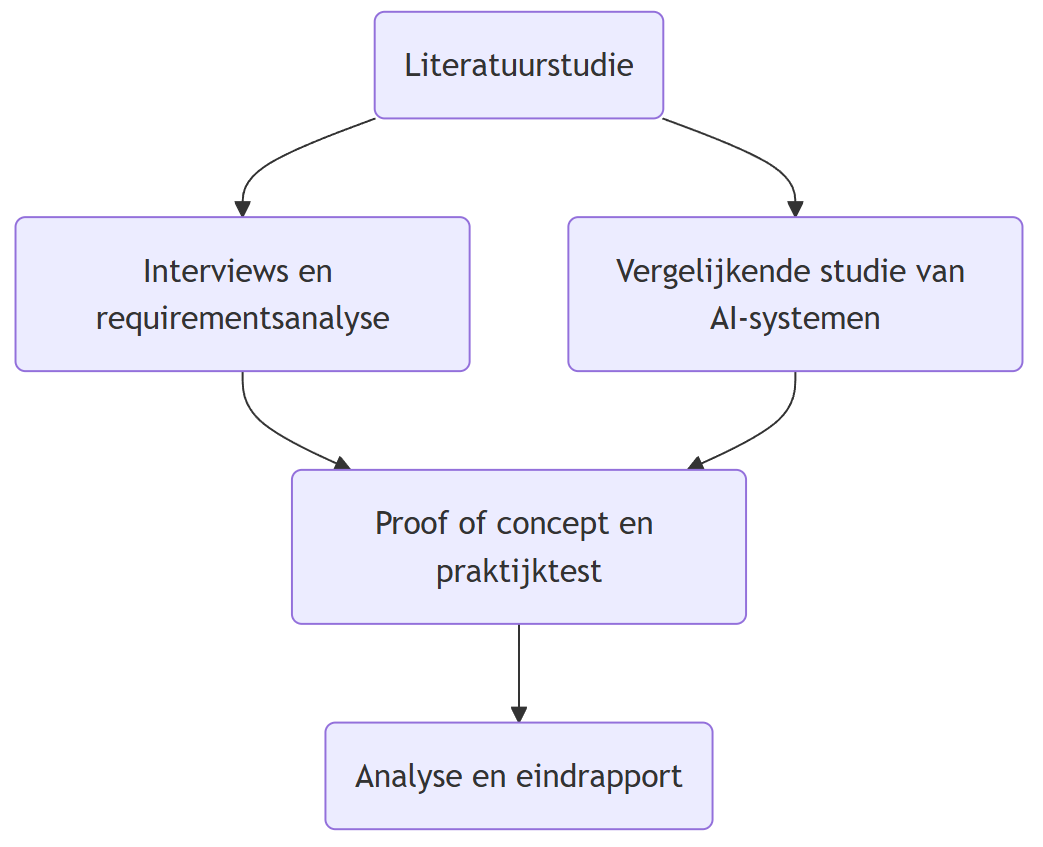
\includegraphics[width=0.3\textwidth]{img/flowchart.png}
  \caption{\label{fig:flowchart}Flowchart bachelorproef}
\end{figure}

%---------- Verwachte resultaten ----------------------------------------------
\section{Verwacht resultaat, conclusie}%
\label{sec:verwachte_resultaten}

Dit onderzoek richt zich op het automatiseren van spelers- en matchstatistieken bij volleybalclub Lindemans Aalst en beoogt een positieve invloed op de nauwkeurigheid en snelheid van dataverzameling, waarmee de club strategisch betere keuzes kan maken. Momenteel worden statistieken tijdens wedstrijden handmatig bijgehouden, terwijl er tijdens trainingen zelfs geen gegevens worden verzameld. Dit handmatige proces is tijdrovend en kan leiden tot inconsistenties in de data. Automatisering biedt potentieel voor een systeem dat in staat is real-time statistieken vast te leggen, zowel tijdens wedstrijden als trainingen, wat resulteert in een meer efficiënte en betrouwbare dataverzameling.

Allereerst wordt een verbetering verwacht in de nauwkeurigheid van gegevensverzameling. Het geautomatiseerde systeem zal naar verwachting 15-25\% nauwkeuriger zijn dan de handmatige methode door het verminderen van menselijke fouten. 

Daarnaast wordt een aanzienlijke tijdsbesparing verwacht in de snelheid van data-analyse. Door een AI-gestuurd systeem toe te passen, wordt voorspeld dat de tijd voor gegevensverwerking en analyse met 30-50\% kan worden verminderd, wat vooral waardevol is tijdens het dynamische wedstrijdmoment. Het systeem zou in staat moeten zijn om gegevens direct beschikbaar te maken, zodat beslissingen tijdens wedstrijden onmiddellijk kunnen worden aangepast aan de real-time prestaties van het team.

Bovendien wordt verwacht dat het systeem de tactische beslissingen en trainingsinzichten van de coaches aanzienlijk zal verbeteren. Met de beschikbaarheid van gedetailleerde statistieken tijdens en na wedstrijden en trainingen zullen coaches in staat zijn om beslissingen te nemen op basis van een hogere kwaliteit en kwantiteit aan data. 

De meerwaarde voor Lindemans Aalst ligt in drie hoofdgebieden: betere en snellere besluitvorming, efficiëntieverbetering en langetermijninzicht. Door real-time inzicht te krijgen in prestaties, zowel tijdens wedstrijden als trainingen, kunnen coaches gefundeerde keuzes maken, tijd besparen en diepgaandere analyses uitvoeren. Het systeem biedt ook meerwaarde door historische gegevens op te slaan, zodat trends en ontwikkeling van spelers goed gevolgd kunnen worden. De resultaten van dit onderzoek bieden niet alleen een waardevolle tool voor Lindemans Aalst, maar verschaffen ook inzichten die andere sportorganisaties kunnen inspireren om AI-technologieën voor datagedreven analyse en besluitvorming te implementeren.
